%Start
%
%
%******************************************************************************************************%
%                                            Mohr's circle                                             %
%******************************************************************************************************%
% Draws Mohr's circle for given stress - values. Input are those stress - values                       %
%******************************************************************************************************%
% Version 1,                                                                                           %
% 29.07.2023                                                                                           %
% L.Lentz@umwelt-campus.de                                                                             %
%******************************************************************************************************%
%
%
\documentclass[tikz,border=10pt]{standalone}
\usetikzlibrary{calc}
%
\begin{document}
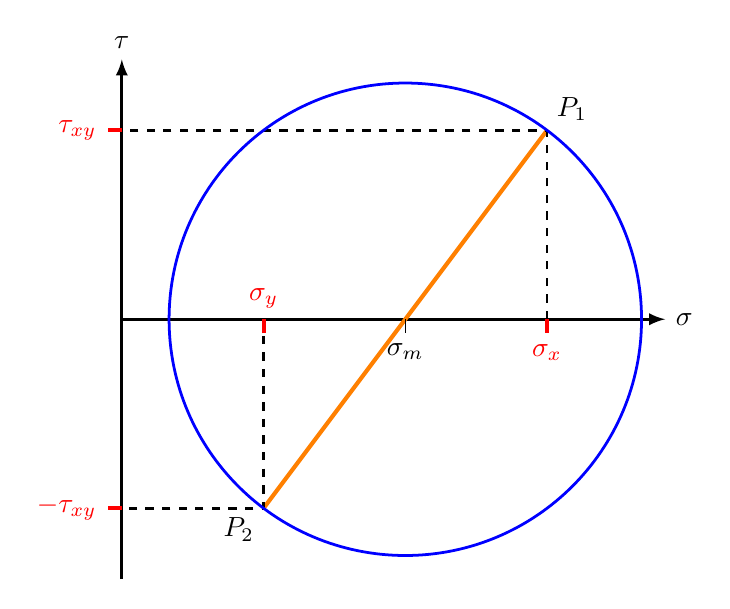
\begin{tikzpicture}[scale=0.6]
%
%
%''''''''''''''''''''''''''''Choose stress values''''''''''''''''''''''''''''''''''''''''''''''''''''''''
\def\sigmax{9}
\def\sigmay{3.}
\def\tauxy{4}
%''''''''''''''''''''''''''''''''''''''''''''''''''''''''''''''''''''''''''''''''''''''''''''''''''''''''
%
\pgfmathsetmacro\sigmam{0.5*(\sigmax+\sigmay)} % compute center of circle
\pgfmathsetmacro\r{sqrt((0.5*(\sigmax-\sigmay))^2+\tauxy^2)} % compute radius of circle
%
\def\s{0.5}; % parameter for small offsets
\pgfmathsetmacro\w{\sigmam+\r+\s}; % parameter for width
\pgfmathsetmacro\h{\r+\s}; % parameter for heigth
%
%\draw[step=0.5,gray] (-4*\s,-\h) grid (\w+\s,\h+\s);% turn on grid if wanted
%
% coordinate system
\draw[line width = 1pt,-latex](0,-\h)--(0,\h)node[at end, anchor = south]{$\tau$};
\draw[line width = 1pt,-latex](0,0)--(\w,0)node[at end, anchor = west]{$\sigma$};
%
% draw connecting line
\draw[color=orange,line width = 1.5pt](\sigmax,\tauxy)--(\sigmay,-\tauxy);
\node at (\sigmax,\tauxy)[anchor=south west]{$P_1$};
\node at (\sigmay,-\tauxy)[anchor=north east]{$P_2$};
%
% draw stress values
\draw[dashed,line width=1.pt](\sigmax,0)--+(0,\tauxy)--(0,\tauxy);
\draw[color=red,line width = 1.5pt](0,\tauxy)--+(-0.3,0)node[anchor = east]{$\tau_{xy}$};
\draw[dashed,line width=1.pt](\sigmay,0)--+(0,-\tauxy)--(0,-\tauxy);
\draw[color=red,line width = 1.5pt](0,-\tauxy)--+(-0.3,0)node[anchor = east]{$-\tau_{xy}$};
\draw[color=red,line width = 1.5pt](\sigmax,0)--+(0,-0.3)node[anchor = north]{$\sigma_x$};
\draw[color=red,line width = 1.5pt](\sigmay,-0.3)--+(0,0.3)node[anchor = south]{$\sigma_y$};
\draw[](\sigmam,0)--+(0,-0.3)node[anchor = north]{$\sigma_m$};
%
%draw circle
\draw[color = blue, line width = 1pt](\sigmam,0) circle (\r);
%
\end{tikzpicture}
\end{document}
%
%
%
%End